\section{Alternatives To HTTP/2}

In determining whether HTTP/2 is likely to increase in popularity in the future, it is important to take a brief look at some competing protocols.

One such protocol that I mentioned previously is called QUIC (Quick UDP Internet Connections)~\cite{quic}. This aims to gain some performance benefits by combining `layers' of protocols. Protocols usually do one specific function, so it is necessary to arrange them in sort of a stack in order to achieve the required functionality. For example, one protocol might be used to ensure that any data that is lost during transmission gets re-transmitted, another protocol might be used to encrypt data, and another protocol (such as HTTP) might be used to determine how to interpret the data that is received. Due to their modularity it is then possible to replace or remove different parts of that protocol stack with ease. A simple analogy for this would be an message in English \hyp{} you could choose to write it down, send it via text, dictate it etc. You could also opt for using a different language, say French. The choice of language is totally independent of the method that is used for transporting the message (and \textit{vice versa}), so any of these components can be swapped at will.

\begin{figure}
	\centering
	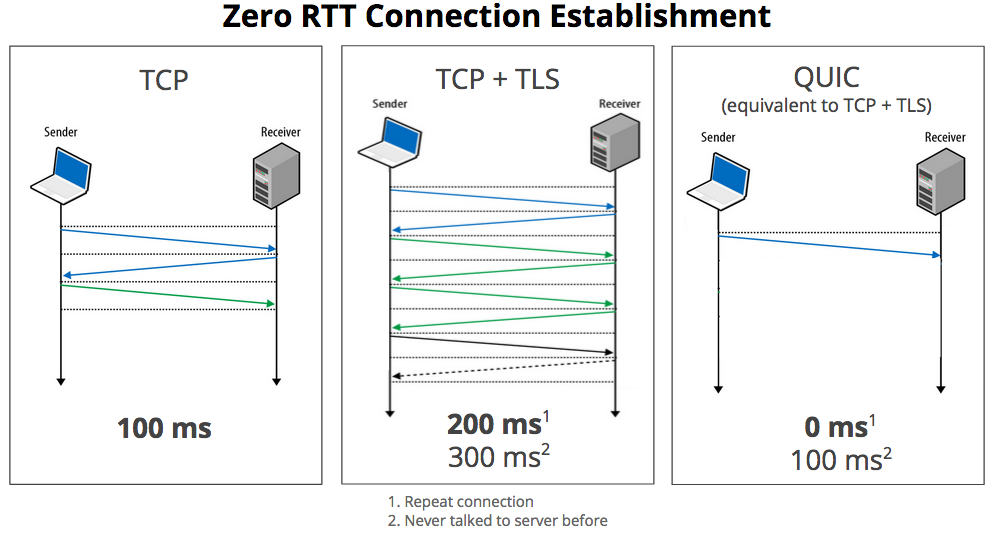
\includegraphics[width=0.6\textwidth]{quic.png}
	\caption{Round trips are decreased significantly in QUIC}
	\label{fig:quic}
\end{figure}

In the case of an encrypted HTTP/2 connection, there are essentially 3 protocols: TCP, TLS and HTTP/2. TCP is a protocol that guarantees that data arrives in the correct order and is re-transmitted if necessary, while TLS handles the encryption and HTTP/2 handles the semantics. QUIC essentially combines these three protocols into one single protocol that still serves the same overall function. By combining them you do lose some modularity but some optimisations can be made as there are some redundant components. I mentioned previously that HTTP/2 has a mechanism for adding `padding' bytes to data that is sent, in order to enhance the security. However TLS also has this mechanism, so it is effectively implemented twice. Another optimisation that can be made is the combination of `handshakes'. A handshake is a pre-defined exchange of information upon initial communication. Each protocol does this differently, with HTTP/2 sending a specific ASCII-encoded string followed by an exchange of settings so that the other end knows which features of the protocol are in use. TCP and TLS both do something similar, however the TLS handshake cannot start until the TCP handshake is complete, and the HTTP/2 handshake cannot start until the TLS handshake is complete. If each handshake is taking a very optimistic 3 round trips, this would add up to 9 round trips in total, which can easily add up to a delay of over a second before any meaningful data is transmitted. Combining these handshakes (as seen in figure \ref{fig:quic}) can therefore lead to significant decreases in delays starting up connections, and through use of some other optimisations the handshake is effectively one round trip. However, as mentioned previously, starting new connections in the context of HTTP/2 is fairly rare anyway so the overall savings that accumulate over many requests are fairly negligible.

There are a number of other reasons why performance is greatly increased in QUIC but the empirical data does show a clear boost in performance. The Google homepage saw a 3.6-8\% drop in search latency and a mean 3\% decrease in the search page load time when using QUIC as opposed to normal HTTP. Google also reports that the slowest 1\% of connections load 1 second faster using QUIC~\cite{quic-look}.

QUIC was initially designed by Google, and adoption of the protocol is fairly unimpressive. The only major browser to support QUIC is Google Chrome and server support for QUIC is around 0.8\% of all websites~\cite{quic-report} making up a respectable 7\% of all internet traffic~\cite{quic-lwn}, with most of the popular websites that support it being ones owned by Google. This is perhaps the largest disadvantage of QUIC compared to HTTP/2 - it is not easy for server operators to add support for it due to the lack of both client and server support. Realistically, only large companies such as Google are going to be able to support such a protocol, at least in the short term while the software ecosystem for QUIC is relatively new.

\iffalse
\subsection{CoAP}

CoAP (Constrained Application Protocol) is a protocol similar to HTTP/2 that is more focused towards small embedded devices suitable for use in the `internet of things' (IoT)~\cite{coap}. As the name may suggest, there is no precise definition of the IoT but it generally refers to networks of small sensors all communicating which can be used in many applications such as smart homes and smart cities. For such a network it is important that the protocol is compact (so that the chance of data being lost due to noise is decreased) and also computationally inexpensive to manage (so that the devices do not expend too much battery during operation). As such there is also less of a focus on performance as there is in HTTP/2.
\fi
